\documentclass[compress,handout,10pt]{beamer}

\newlength{\wideitemsep}
\setlength{\wideitemsep}{\itemsep}
\addtolength{\wideitemsep}{100pt}
\let\olditem\item
\renewcommand{\item}{\setlength{\itemsep}{0.5\baselineskip}\olditem}

\usetheme{berlin}
\usecolortheme{orchid}
\usefonttheme[onlymath]{serif}

\setbeamertemplate{bibliography item}[text]
\usepackage{float}
%\floatstyle{boxed}
\usepackage{colortbl}
\usepackage{mathpazo}
\usepackage{graphicx}
\graphicspath{{./extra/}}
\usepackage{movie15}
\usepackage{bm}
\usepackage{verbatim}
\usepackage{comment}
\usepackage [font=small, labelfont=bf]{caption}
\usepackage{subcaption}
%\captionsetup[subfigure]{labelformat=empty}
\captionsetup[figure]{labelformat=empty}

\newcommand{\mygreen}{\color{green!50!black}}
\newcommand{\myblue}{\color{blue}}
\newcommand{\myred}{\color{red}}
\newcommand{\mycolor}{\color{red}{c}\color{blue}{o}\color{green}{l}\color{orange}{o}\color{cyan}{r}}
\newcommand{\mysize}{\scriptsize{s}\small{i}\normalsize{z}\Large{e}}
\newcommand{\myshape}{\textcircled{s}\textit{h}\texttt{a}\textsf{p}\textsc{e}}

%\xdefinecolor{titlecolor}{rgb}{.855,.647,.125}
%\xdefinecolor{titlecolor}{rgb}{0,0,0}
%\setbeamercolor{frametitle}{fg=titlecolor}
\setbeamerfont{frametitle}{series=\bfseries}
\setbeamercolor{normal text in math text}{parent=math text}

\setbeamertemplate{navigation symbols}{} %gets rid of navigation symbols
\setbeamertemplate{footline}[frame number]
\beamertemplateshadingbackground{blue!5}{yellow!10}

\title{{\LARGE Modeling and Simulating Fan Participation at Large Scale Sporting Events\newline} }

\subtitle{{\large Blue Jays Unlimited} }

\author{ 
%    \vspace{5pt}
    {\bf{Presenter:}} \\ 
Steven Su \\ 
    \vspace{5pt}
} 
\institute{JHU AMS 550.400 Fall 2012}

\date{Last Complied on \today} 

\begin{document}

\begin{frame}[plain]
    \titlepage
\end{frame}

\begin{frame}
    \frametitle{Overview}
    {\small \tableofcontents}
\end{frame}

\section{Introduction}

\subsection{Participants and Sponsors}

\begin{frame}
	\frametitle{Participants and Sponsors}
	\begin {itemize}
		\item Student participants:
			\begin {itemize}
				\item Steven Su
				\item Danni Tang
				\item Ahmed Aly
			\end {itemize}
		\item Sponsor: Blue Jays Unlimited	
	\end {itemize}
\end{frame}

\subsection{Sponsor Information}

\begin{frame}
    \frametitle{Who are Blue Jays Unlimited?}
    \begin {columns}
    	\begin{column}{0.5\textwidth}
    		\begin {itemize}
    			\item Blue Jays Unlimited (BJU) was established in 1995 \cite{bjuwebsite}
    			\item Volunteer group of over 3000 alumni, friends, and staff, based in Baltimore, MD, dedicated to supporting and promoting Johns Hopkins University (JHU) athletics \cite{bjuwebsite}
    			\item Official booster club for JHU athletics \cite{bjuwebsite}
    		\end {itemize}
    	\end {column}
    	\begin {column}{0.5\textwidth}
    	\begin{figure} [h]
    		\begin{center}
    			
\includegraphics [width=2in] {BJU.jpg}
    			\caption {{\tiny The logo of Blue Jays Unilimited. \textit{Courtesy of: http://www.hopkinssports.com/bluejays-unlimited/}}}
    		\end{center}
    	\end {figure}	
    	\end {column}
    \end{columns}
\end{frame}

\begin{frame}
	\frametitle{What Does BJU do for Hopkins?}
	\begin {columns}
		\begin {column} {0.5\textwidth}
			\begin {itemize}
				\item Raised more than \$4 million in funds to improve experience for JHU student athletes and fans alike \cite{bjuwebsite}
				\item Funds provide money for capital projects as well as scholarships and operational endowments \cite{bjuwebsite}
				\item Past projects include renovation of the Newton H.~White Athletic Center and recognition banners for championship teams. \cite{bjuwebsite}
			\end {itemize}
		\end {column}
		\begin{column} {0.5\textwidth}
			\begin{figure}
			\begin{center}
				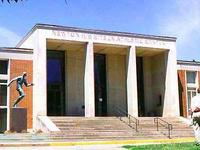
\includegraphics [width=2in] {AthleticCenter.jpg}
				\caption{{\tiny The Newton H.~White Athletic Center after renovations. \textit{Courtesy of: http://events.jhu.edu/WhiteAthleticCenter\#.UHhNK1GRWSo}}}
			\end{center}
			\end {figure}
		\end {column}
	\end {columns}
\end {frame}   

\begin{frame}
    \frametitle{BJU at Sporting Events}
    \begin{itemize}
    	\item BJU is present at nearly all major JHU sporting events
    	\item Encourage fans to cheer on their Blue Jays to victory in a vociferous and family-friendly manner
    	\item BJU's goal is to provide Hopkins' teams with the ultimate advantage: a spirited home crowd
    \end{itemize}
\end{frame}

\section{Problem Statement}

\subsection{Problem Statement Background}

\begin{frame}
	\frametitle{Problem Statement Background: Why is Cheering Important?}
		\begin{itemize}
			\item A loud and supportive home crowd is the ultimate home team advantage to any collegiate sports team. 
			\item Fan participation in events such as chanting the school fight song, waving a rally towel, doing the wave, or general applause, show support for the home team as well as enhance the general atmosphere of a sporting event. 
			\item Note that we will hence refer to all these activities as ``cheering''.
		\end{itemize}
\end{frame}

\begin{frame}
	\frametitle{Problem Statement}
			\begin {itemize}
				\item BJU is interested in maximizing cheering at Homewood Field located on the Homewood campus of JHU in Baltimore, MD. 
				\item BJU believes that they can increase cheering by placing ``cheer starters'' in the home crowd.
				\item ``Cheer starters'' are student volunteers who urge other fans around them to cheer. 
			\end {itemize}
\end{frame}

\subsection{Official Problem Statement}

\begin{frame}
	\frametitle{Official Problem Statement}
	\begin{itemize}
		\item BJU wants to know if ``cheer starters'' can actually increase cheering and also want a simple model of fan participation in cheering.
	\end{itemize}
\end{frame}

\section {Objectives}

\subsection{Important Details to Consider}

\begin{frame}
	\frametitle {Important Details To Consider}
		\begin {columns}
			\begin {column}{0.5\textwidth}
				\begin{itemize}
					\item Homewood Field's capacity is approximately 8500 spectators \cite{wiki}
					\item Long rectangular section of the bleachers in the lower left is traditionally reserved for Blue Jays' fans and seats approximately 4000 fans.
				\end {itemize}
			\end {column}
			\begin {column}{0.5\textwidth}
			\begin {figure}
				\begin{center}
    			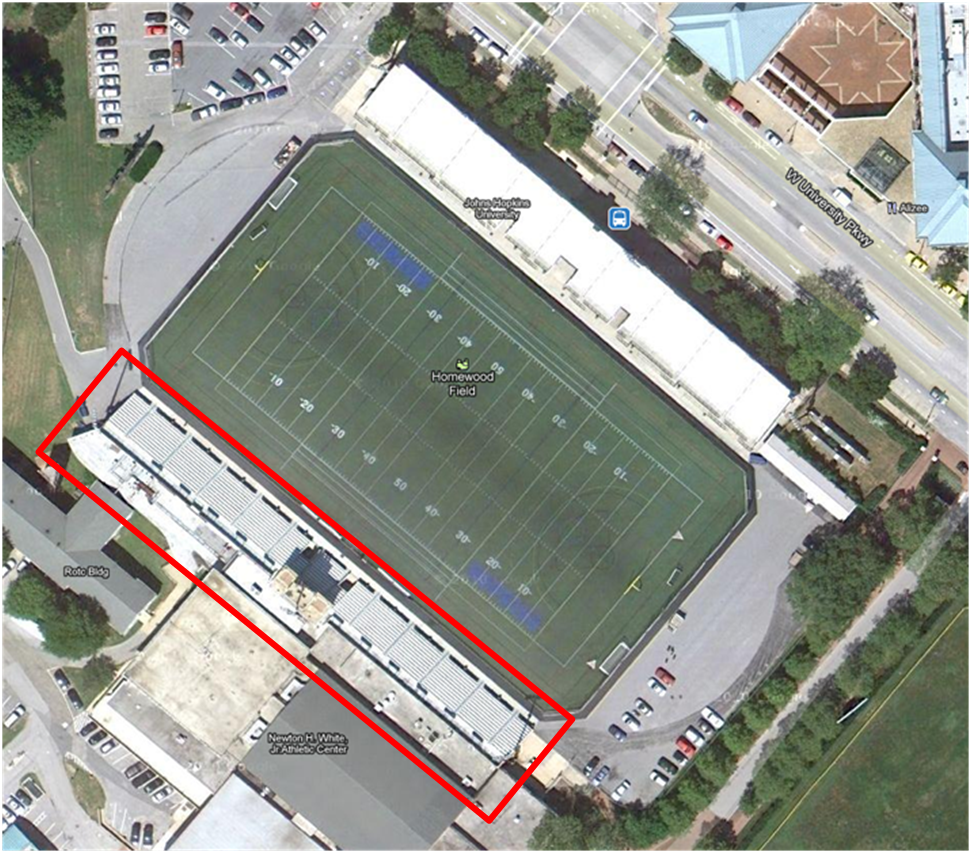
\includegraphics [width=2in] {Bleachers.png}
    			\caption {{\tiny A satellite image of Homewood Field. The home team bleachers are highlighted in red. \textit{Courtesy of: www.google.com}}}
    		\end{center}
    	\end{figure}	
			\end {column}
		\end {columns}
\end{frame}

\begin{frame}
	\frametitle{Important Details to Consider}
		\begin{itemize}
			\item Home bleachers are usually filled to capacity for all major Hopkins sporting events
			\item Because of how fans normally sit, BJU is specifically interested in maximizing cheering in the home team bleachers
		\end{itemize}
\end{frame}

\subsection{Official Objectives}

\begin{frame}
	\frametitle {Official Objectives}
	\begin {itemize}
		\item Our task is to provide BJU with a simple model of fan participation in cheering at Homewood Field in the home team bleachers as well as simulation results from the model which determine if their belief about cheer starters is accurate. 
		\item If cheer starters are found to be effective, we will attempt to provide BJU with more details about the quantity and location at which cheer starters should be placed in order to maximize cheering.
	\end {itemize} 
\end{frame}

\section {Approach}

\subsection {Overview}

\begin {frame}
	\frametitle {Overview of Entire Model}
	\begin{itemize}
		\item Two models will be created: single fan model and multi fan model
		\item Single fan model will be stochastic in nature and will determine if a single fan starts to cheer
		\item Multi fan model will use the single fan model to simulate a large crowd of fans
	\end{itemize}
\end {frame}

\subsection{Single Fan Model}

\begin {frame}
	\frametitle {A Model for a Single Fan: General Parameters}
	\begin{itemize}
		\item Stochastic model will use serveral parameters/variables to calculate a \emph{cheering metric}, $C_{Total}$, which determines whether a fan will participate in cheering
		\begin{itemize}
			\item Fan's innate level of support of the team
			\item Number of fans around a given fan who are cheering
			\item Threshold of cheering 
		\end{itemize}
	\end {itemize}
\end {frame}

\begin {frame}
	\frametitle{A Model for a Single Fan: Fan's Innate Level of Support for Team}
	\begin{itemize}
		\item The greater the level of support a fan has for a team, the more likely he/she will cheer his/her team on.
		\item Model for single fan is stochastic in that the support level for the team will be randomized between fans
		\item This more accurately reflects reality where different fans can have different levels of support for the same team.
	\end{itemize}
\end {frame}

\begin{frame}
	\frametitle{A Model for a Single Fan: Fan's Innate Level of Support for Team}
	\begin {columns}
		\begin {column} {0.5\textwidth}
			\begin{itemize}
				\item Currently thinking of using a Normal Distribution (a bell curve) to randomly assign a score to represent a fan's innate support level.
				\item The majority of fans who go to sporting events are average fans who go to games because they like the team. A smaller proportion of fans at sporting events are are fanatics for the team. A smaller proportion are also spectators who don't care for the team.
			\end{itemize}
		\end {column}
		\begin {column} {0.5\textwidth}
		\begin{figure}
		\begin{center}
			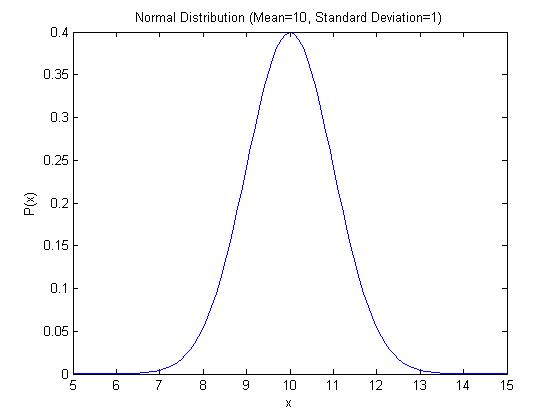
\includegraphics [width=2in] {NormDistribution.jpg}
			\caption{{\tiny MATLAB plot of a normal distribution with a mean of 5 and a standard deviation of 1.}}
		\end{center}
		\end{figure}
		\end {column}
	\end {columns}	
\end{frame}

\begin {frame}
	\frametitle {A Model for a Single Fan: Number of Fans Surrounding a Fan Who Are Cheering}
		\begin{itemize}
			\item The more people surrounding a fan who are cheering, the more likely the fan is to join the cheering
			\item Will scale a given fan's innate support level score by the number of adjacent fans around the given fan who are cheering
		\end {itemize}
\end {frame}

\begin {frame}
	\frametitle {A Model for a Single Fan: Cheering Metric ($C_{Total}$) and Cheering Threshold ($C_{Threshold}$)}
	\begin{itemize}
		\item Considering to define $C_{Total}$ as follows: \newline
	\end {itemize}
	$$C_{Total} = (Innate\ Support\ Level)(Number\ of\ Adjacent\ Fans\ Who\ Are\ Cheering)$$
	\begin{itemize}
		\item The following condition must be satisfied for start cheering:\newline
	\end {itemize}	
	$$C_{Total}>C_{Threshold}$$
	\begin{itemize}
		\item $C_{Threshold}$ is an arbitrary pre-defined parameter
	\end {itemize}
\end {frame}


\subsection{Multi Fan Model}

\begin{frame}
\frametitle {Multi Fan Model: Matrix Representation of a Crowd}
	\begin {itemize}
		\item Considering the use of matrices to represent a large crowd of fans
		\item Each element in a matrix will represent a fan
		\item One matrix will store each fan's $C_{Total}$ value, another will store each fan's innate support level score, and another will keep track of which of the fans in the crowd are cheering 
	\end{itemize}		
\end{frame}

\begin{frame}
\frametitle {Multi Fan Model: Matrix Representation of a Crowd}
	\begin {itemize}
		\item Matrices will be long and rectangular to reflect the spatial arrangement of the home team bleachers at Homewood Field
		\item Due to computatational limits, we will downscale the home team bleachers at Homewood Field and model a home crowd of 100-1000 people
	\end{itemize}		
\end{frame}

\begin{frame}
\frametitle{Multi Fan Model: Simulation of Time (Cycling)}
To simulate the passing of time:
	\begin {enumerate}
		\item Setup matrices with appropriate initial conditions (i.e.~randomly assign innate support levels to each fan and choose quantity and location of cheer starters)
		\item Check to see if any new fans join cheering
		\item Update matrices
		\item Repeat for 10 cycles
	\end {enumerate}
\end{frame}

\begin{frame}
\frametitle{Multi Fan Model: Simulation of Time (Cycling)}
	\begin {itemize}
		\item Each cycle will represent the passing of 3-5 seconds
		\item We will assume that once a fan starts cheering, he/she will continue cheering until the end of the simulation
	\end{itemize}
\end{frame}	

\begin{frame}
\frametitle{Multi Fan Model: Determining if Cheer Starters Increase Cheering}
\begin{itemize}
	\item Repeatedly run the previously described simulation (Monte Carlo methods) and get an average percentage of fan participation in cheering for a given cheer starter setup
	\item Compare this to simulation results with no cheer starters
	\item Time permitting, will try using Monte Carlo methods for various cheer starter setups and attempt to identify any patterns in setups which maximize cheering 
\end{itemize}
\end{frame}

\section {Deliverables and Timeline}

\subsection{Deliverables}

\begin{frame}
	\frametitle{Deliverables}
	The model will be coded on MATLAB R2009b. All computations will be performed on a Intel Core i7 Desktop PC. \newline
	\end{frame}

\begin{frame}
	\frametitle{Deliverables}
	From Team to Sponsor:
	\begin {itemize}
	\item MATLAB R2009b and R combination package. The model will be coded in MATLAB but a complete set of documentation will be provided in R. We will also generate some test scripts that can be used to reproduce our numerical and simulation test results
	\item If time permits, a list of patterns of cheer starter setups (i.e.~the number of cheer starters and location of them) that maximize fan cheering
	\item Technical report and presentations summarizing the work \newline
	\end{itemize}
\end{frame}

\begin{frame}
	\frametitle{Deliverables}
	From Sponsor to Team:
	\begin{itemize}
		\item Timely responses to inquiries
	\end{itemize}
\end{frame}

\subsection{Timeline}

\begin{frame}
	\frametitle{Timeline of Milestones}
	\begin{itemize}
    \item Work Statement due date, Sep 28, 2012.
    \item Midterm Presentation due date, Oct 17, 2012.
    \item Progress Report due date, Oct 26, 2012.
    \item Final Presentation due date, Nov 16, 2012.
    \item Final Report due date, Nov 30, 2012.
	\end{itemize}
\end{frame}

\section{Conclusion}

\subsection{Work Remaining to Be Done}

\begin{frame}
	\frametitle{Remaining Work}
	\begin {itemize}
		\item Begin coding the model in MATLAB.
		\item Run simulations using the model.
		\item Time permitting, try to find patterns in cheer starter setups which maximize cheering.
	\end {itemize}
\end{frame}

\subsection{Recommendations for Future Research}

\begin{frame}
	\frametitle {Recommendations for Future Research}
	\begin {itemize}
		\item It would be interesting to see if this model could be applied to other social events (concerts, college lectures, theaters, etc.) where there are large crowds and applause is relevant.
	\end {itemize}
\end{frame}

\subsection{}

\begin {frame}
	\frametitle{References}
	\bibliographystyle{plain}
	%\nocite{*}
	\bibliography{extra/biblioWS}
\end {frame}

\begin{frame}
	\frametitle {Questions?}
	\begin{center}
		Questions?
	\end{center}
\end{frame}

\end{document}
